\documentclass[12pt]{article}

\usepackage[margin=1in]{geometry}
\usepackage{amssymb, amsmath, amsfonts, bm, graphicx, geometry}
\usepackage{tabularx, booktabs, float, enumitem, multicol, mathtools}
\usepackage{parskip} % Auto-manages paragraph spacing and removes indentations
\usepackage{siunitx}  % Eases typesetting of numbers and units
\usepackage{soul}
\usepackage{mathrsfs}
\title{ME352 QUBE Motor Lab 2\\Motor Speed PI Control}
\author{Zeshui Song}
\date{October 2, 2026}

\begin{document}

\maketitle

\section{Overview}
In this lab we will apply feedback control to the QUBE DC motor system with the goal of acceptable transient response and tracking. Proportional control (P) offers the advantage of fast transient response and reducing steady state error. While higher gains yield better performance, they come at the expense of increased sensitivity to noise. We will learn that integral control (I) offers the advantage of zero steady-state error for a step input to this system. (This is not generally true for all systems). Unfortunately, however, as the gain of I is increased to improve rise time, overshoot and instability will also increase. We will see that combining P and I (PI control) is better than either P or I alone by simultaneously offering the advantages of quick transient response, zero steady-state error and decreased sensitivity to noise.

\section{Goals}
Our hands-on goals for this lab are to:
\begin{itemize}
    \item Learn how to work as a designer. Use a model of the DC motor system to design a suitable controller which is implemented in an experiment.
    \item Design a feedback controller for reference tracking using P, I, and PI control approaches.
    \item Compare measured responses to those simulated for the modeled system.
\end{itemize}

\section{Pre-lab Questions}
Come prepared to your scheduled lab session with the pre-lab questions answered. Turn in the pre-lab questions with the lab assignment.
\subsection*{Transfer Function Derivation}
\textbf{Schematic}
\begin{center}
    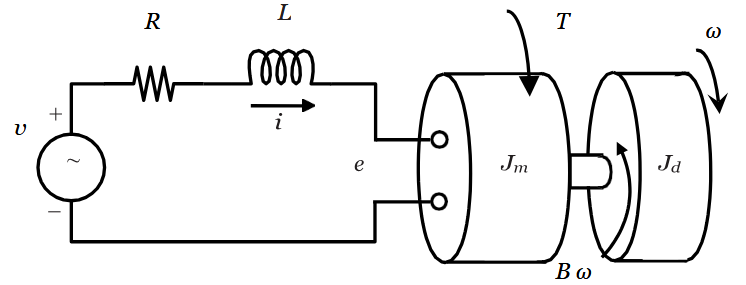
\includegraphics[width=0.65\textwidth]{Schematic.png}
\end{center}
Where:
\begin{itemize}
    \item $e = k_b \omega$ is the back EMF voltage (law of the generator)
    \item $T = k_m i$ is the torque generated by the motor (law of the motor)
\end{itemize}
\textbf{Equations of Motion}\\
Assuming a rigid connection between the motor and the load disc, the equations of motion for the system are:\\\\
KVL:
\[L \frac{di}{dt} + Ri +e = V \quad \implies \quad L \frac{di}{dt} + Ri +k_b \omega = V\]
Sum of torques (Newton):
\[J \frac{d \omega}{dt} + B\omega = T \quad \implies \quad J \frac{d \omega}{dt} + B\omega = k_m i\]
Where $J = J_m + J_d$ is the total inertia of the system.\\\\
\textbf{Laplace Transform}\\
With zero initial conditions since we are solving for the transfer function:
\[L(sI(s))+RI(s) + k_b \Omega(s) = V(s) \quad \implies \quad I(s) = \frac{V(s) - k_b \Omega(s)}{Ls + R}\]
\[J(s\Omega(s)) + B\Omega(s) = k_m I(s)\]
Plug in for $I(s)$:

\[J(s\Omega(s)) + B\Omega(s) = k_m \frac{V(s) - k_b \Omega(s)}{Ls + R}\]
Rewrite:
\[Js\Omega(s)(Ls+R) + B\Omega(s)(Ls+R) = k_mV(s) - k_mk_b \Omega(s)\]
\[(JLs^2 +JRs)\Omega(s) + (BLs + BR)\Omega(s) + k_mk_b \Omega(s) = k_mV(s)\]
\[\boxed{\implies G(s) = \frac{\Omega (s)}{V(s)} = \frac{k_m}{JLs^2 + (JR+BL)s+(BR + k_mk_b)} \quad \text{(transfer fxn)}}\]
\subsection*{Parameter Identification}
Recall from lab 1 that the first-order transfer function of the motor plant is given by:
\[P(s) = \frac{K}{\tau s + 1}\]
\textbf{1.} Write down the calculated values for $K$ and $\tau$ you determined in lab 1, including units, using the QUBE-Servo manufacturer values of
\begin{itemize}
    \item Motor resistance, $R = 8.4~\Omega$,
    \item Motor inertia (includes the hub attachment inertia), $J_m = 4.65\times10^{-6}~\mathrm{kg\,m^2}$,
    \item Motor torque constant, $K_m = 0.042~\mathrm{N\,m/A}$,
    \item Motor back EMF constant, $K_b = 0.042~\mathrm{V/(rad/s)}$.
\end{itemize}
To calculate the load disc inertia, $J_d$, assume the disc has a mass of $0.053~\mathrm{kg}$ and radius of $0.0248~\mathrm{m}$. Assume the motor damping/friction and the armature inductance are negligible.\\\\
\textbf{Assumptions for a first order system}
\begin{itemize}
    \item Neglect the motor inductance, $L=0$.
    \item Neglect the motor damping/friction, $B=0$.
\end{itemize}
\[G(s) = \frac{k_m}{JRs+ k_mk_b}\]
Compare to the form of a first-order transfer function:
\[G(s) = \frac{K}{\tau s + 1} = \frac{k_m}{JRs+ k_mk_b} = \frac{\frac{k_m}{k_m k_b}}{\frac{JR}{k_m k_b}s+1}\]
Thus:
\begin{itemize}
    \item DC gain:
    \[K = \frac{k_m}{k_m k_b} = \frac{1}{k_b}\]
    \item Time constant:
    \[\tau = \frac{JR}{k_m k_b}\]
\end{itemize}
\textbf{Solve for $J_d$}
\[J_d = \frac{1}{2}m_d r_d ^2  = \frac{1}{2}[0.053~\mathrm{kg}][0.0248~\mathrm{m}]^2 = 1.629 \times 10^{-5}~\mathrm{kg\,m^2}\]
\[\implies J = J_m + J_d = [4.65\times10^{-6}~\mathrm{kg\,m^2}] + [1.629 \times 10^{-5}~\mathrm{kg\,m^2}] = 2.094 \times 10^{-5}~\mathrm{kg\,m^2}\]
\newpage
\textbf{Plug in and solve for parameters}
\begin{itemize}
    \item DC gain:
    \[K = \frac{1}{k_b} = \frac{1}{[0.042~\mathrm{V/(rad/s)}]} = \boxed{23.809~\mathrm{(rad/s)/V}}\]
    \item Time constant:
    \[\tau = \frac{JR}{k_m k_b} = \frac{[2.094 \times 10^{-5}~\mathrm{kg\,m^2}][8.4~\Omega]}{[0.042~\mathrm{N\,m/A}][0.042~\mathrm{V/(rad/s)}]} = \boxed{0.0997~\mathrm{s}}\]
\end{itemize}
\subsection*{Proportional (P), Integral (I) and Proportional-Integral (PI) Control}
A common block diagram for reference tracking is shown in Fig.~1. Recall that a proportional-integral controller has transfer function:
\[C(s) = k_p + \frac{k_i}{s}\]
\begin{figure}[H]
    \centering
    \includegraphics[width=0.65\textwidth]{Block dia.png}
    \caption{Block diagram for error-based feedback control (reference tracking).}
\end{figure}

In the following, we consider proportional, integral and proportional-integral control for the motor-tachometer system. For all three types of control our goal is to design a controller such that:

\begin{enumerate}
    \item[(i)] the rise time is less than $0.2$ seconds,
    \item[(ii)] the steady-state error is less than $1\%$,
    \item[(iii)] the overshoot is less than $20\%$,
    \item[(iv)] the noise in the input signal (applied motor voltage) is small. The spread of the amplitude with respect to the mean signal should be less than $0.25$ volts.
\end{enumerate}

You, the control designer, need to find out if you can meet all prescribed specifications.

For this lab, use the approximation that rise time from $10$--$90\%$ of steady-state is

\[
t_r \approx \frac{1.8}{\omega_n}.
\]

Note this is only a \hl{rough approximation based on the behavior of second-order systems with no zeros}. For first-order systems, the transient behavior can be better characterized by the time constant, which is related to the pole location.

You may recall or will learn that overshoot is
\[
M_p(\zeta)= \frac{y_\text{peak} - y_\text{ss}}{y_\text{ss}}
=
e^{-\pi\zeta/\sqrt{1-\zeta^2}},
\]
which approximately yields $\zeta > 0.5$ for $M_p < 20\%$.\\\\
Note the form:
\[\frac{s}{s^2 +2\zeta \omega_n s + \omega_n^2},\quad \frac{\omega_n^2}{s^2 +2\zeta \omega_n s + \omega_n^2}\]
\begin{center}
    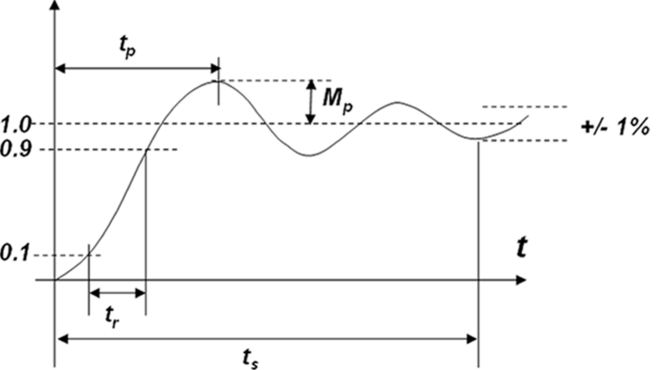
\includegraphics[width=0.65\textwidth]{Time specs.png}
\end{center}
\subsection*{Proportional Control}
First, we consider proportional control, i.e.
\[
C(s)=k_p.
\]
\textbf{2.} Use the final value theorem and reference-to-error transfer function, or determine the error from system type and error constants, to write the steady-state error to a unit step input in terms of the system parameters $K$ and/or $\tau$ and the proportional control constant $k_p$.\\\\
\textbf{Error Transfer Function:}
\[\frac{E(s)}{R(s)}=\frac{1}{1+C(s)P(s)} = \frac{1}{1 + \frac{k_p K}{\tau s+1}}\]
\[\frac{E(s)}{R(s)}=\frac{\tau s+1}{\tau s+1 + k_p K}\]
Final value theorem with a unit step input:
\[R(s) = \frac{1}{s}\]
\[\lim_{t\to\infty} e(t) = \lim_{s\to 0} sE(s) = \lim_{s\to 0} \left(s \cdot \frac{\tau s+1}{\tau s+1 + k_p K}\cdot \frac{1}{s}\right) = \boxed{\frac{1}{1 + k_p K}}\]
\textbf{3.} Design P-controllers such that the steady state error is respectively less than $30\%$, $10\%$, and $1\%$. Calculate the respective ranges of $k_p$ values to meet each steady-state error specification.\\\\
The steady-state error is given by
\[e_{ss} = \frac{1}{1 + k_p K}\]
Since this was derived for a unit step input ($r_{ss} = 1$), the percentage of steady-state error is
\[\%e_{ss} = \frac{y_{ss} - r_{ss}}{r_{ss}} \cdot 100 = \frac{e_{ss}}{r_{ss}} \cdot 100 = e_{ss} \cdot 100\]
\begin{itemize}
    \item For $e_{ss} < 30\%$:
    \[\frac{1}{1 + k_p K} < 0.3 \implies 1 + k_p K > \frac{1}{0.3} \implies \boxed{k_p > \frac{7}{3K}  = 0.098~\mathrm{V/(rad/s)}}\]
    \item For $e_{ss} < 10\%$:
    \[\frac{1}{1 + k_p K} < 0.1 \implies 1 + k_p K > \frac{1}{0.1} \implies \boxed{k_p > \frac{9}{K} = 0.378~\mathrm{V/(rad/s)}}\]
    \item For $e_{ss} < 1\%$:
    \[\frac{1}{1 + k_p K} < 0.01 \implies 1 + k_p K > \frac{1}{0.01} \implies \boxed{k_p > \frac{99}{K}=4.158~\mathrm{V/(rad/s)}}\]
\end{itemize}
\textbf{4.} Find the closed-loop pole and closed-loop time constant for the $k_p$ value corresponding to $1\%$ steady-state error.\\\\
\textbf{Closed Loop Transfer Function}
\[\frac{Y(s)}{R(s)} = \frac{C(s)P(s)}{1+C(s)P(s)} = \frac{\frac{k_p K}{\tau s+1}}{1+\frac{k_p K}{\tau s+1}} = \frac{k_p K}{\tau s+1+k_p K}\]
\textbf{Pole}
\[\tau s+1+k_p K = 0 \implies \boxed{s = -\frac{1+k_p K}{\tau}}\]
For $k_p$ corresponding to $1\%$ steady-state error, $k_p = 99/K$:
\[s = -\frac{1+99}{\tau} = \boxed{-\frac{100}{\tau}}\]
\textbf{Closed Loop Time Constant}\\
Comparing the closed loop transfer function with the form of a first-order system:
\[\frac{Y(s)}{R(s)} = \frac{k_p K}{\tau s+1+k_p K} = \frac{K_{cl}}{\tau_{cl} s + 1}\]
\[\implies \tau_{cl} = \frac{\tau}{1+k_p K} = \boxed{\frac{\tau}{100}}\]
Recall that the plant/open loop time constant is $\tau = 0.0997~\mathrm{s}$ from earlier.
\subsection*{Proportional-Integral Control}
In the proportional-integral controller case,
\[
C(s)=k_p+\frac{k_i}{s},
\]
we can combine the favorable features of both P and I control, namely quick response, zero steady state error, and low sensitivity to noise.\\\\
\textbf{5.} Find the closed-loop transfer function for P-I control. Which property of the closed-loop system is influenced by $k_p$? Similarly, for $k_i$?\\\\
\textbf{Closed Loop Transfer Function}
\[C(s)P(s) = \left(k_p+\frac{k_i}{s}\right) \frac{K}{\tau s+1} = \frac{K(k_p s+k_i)}{s(\tau s+1)}\]
\[\frac{Y(s)}{R(s)} = \frac{C(s)P(s)}{1+C(s)P(s)} = \frac{\frac{K(k_p s+k_i)}{s(\tau s+1)}}{1+\frac{K(k_p s+k_i)}{s(\tau s+1)}}=\frac{K(k_p s+k_i)}{s(\tau s+1)+K(k_p s+k_i)}\]
\[\boxed{\frac{Y(s)}{R(s)} =\frac{Kk_p s+ Kk_i}{\tau s^2+(1+Kk_p) s + Kk_i}}\]
Compare the demoninator with the standard form of a second-order system:
\[\tau s^2+(1+Kk_p) s + Kk_i = s^2 + 2\zeta \omega_n s + \omega_n^2\]
Thus,
\[\boxed{\omega_n = \sqrt{\frac{Kk_i}{\tau}}}\]
\[\zeta = \frac{1+Kk_p}{\tau}\cdot\frac{1}{2\omega_n} =\frac{1+Kk_p}{2\tau} \cdot \sqrt{\frac{\tau}{Kk_i}}\]
\[\boxed{\zeta  =\frac{1+Kk_p}{2\sqrt{\tau Kk_i}}}\]
So $k_p$ primarily affects the damping ratio, $\zeta$, and $k_i$ primarily affects the natural frequency, $\omega_n$. Both gains affect the stability of the system.\\\\
\textbf{6.} For your PI-controller design, find the range of $k_p$ and $k_i$ values that meet or exceed the rise time $t_r \leq 0.2~\mathrm{s}$, overshoot $M_p \leq 20\%$, and steady-state error less than $1\%$.\\\\
Note, if you did the calculations correctly, you should see the $k_p$ gain required to meet the specifications using P-control only is much higher than in the PI-control case. In fact, the theoretical calculations should reveal that you should be able to meet specifications (i)--(iii) with I-control only. During the lab we will see if this is possible in practice.\\\\
\textbf{Rise Time}\\
Using the approximation for a 10--90\% rise time:
\[t_r \approx \frac{1.8}{\omega_n} \leq 0.2 \implies \omega_n \geq 9~\mathrm{rad/s}\]
\[\implies \frac{Kk_i}{\tau} \geq 81 \implies \boxed{k_i \geq \frac{81\tau}{K}}\]
Plugging in the values for $\tau$ and $K$:
\[\implies k_i \geq \frac{[81~\mathrm{(rad/s)^2}][0.0997~\mathrm{s}]}{[23.809~\mathrm{(rad/s)/V}]} = \boxed{0.339~\mathrm{V/rad}}\]
\textbf{Overshoot}\\
The lab says that an overshoot of less than $20\%$ corresponds to a damping ratio of $\zeta > 0.5$. Thus:
\[\zeta  =\frac{1+Kk_p}{2\sqrt{\tau Kk_i}} > 0.5\]
\[1+Kk_p > \sqrt{\tau Kk_i}\]
\[\boxed{k_p > \frac{\sqrt{\tau Kk_i}-1}{K}}\]
\textbf{Steady State Error}\\
The error transfer function is
\[\frac{E(s)}{R(s)} = \frac{1}{1+C(s)P(s)}=\frac{1}{1+\frac{K(k_p s+k_i)}{s(\tau s+1)}} = \frac{s(\tau s+1)}{s(\tau s+1)+K(k_p s+k_i)}\]
Final value theorem with a unit step input $R(s) = \frac{1}{s}$:
\[\lim_{t\to\infty} e(t) = \lim_{s\to 0} sE(s) = \lim_{s\to 0} \left(s \cdot \frac{s(\tau s+1)}{s(\tau s+1)+K(k_p s+k_i)} \cdot \frac{1}{s}\right) = \frac{0}{Kk_i} =\boxed{0}\]
Thus, the steady-state error is zero for a PI-controller, and the $k_p$ and $k_i$ gains can be chosen to meet the rise time and overshoot specifications.
\newpage
\textbf{Using Only $k_i$}\\
It is possible to meet the specifications using only $k_i$:
\begin{itemize}
    \item Rise time: $k_i \geq 0.339~\mathrm{V/rad}$
    \item Overshoot: 
    \[k_p = 0 \implies \quad \frac{1}{2\sqrt{\tau Kk_i}} > 0.5 \implies k_i< \frac{1}{\tau K}\]
    \[k_i < \frac{1}{[0.0997~\mathrm{s}][23.809~\mathrm{(rad/s)/V}]} = \boxed{0.421~\mathrm{V/rad}}\]
    \item  Steady-state error: $e_{ss} = 0$ for any $k_i > 0$
\end{itemize}
\section{Lab Assignment: Tracking the Motor Speed}
The theoretical motor model used for the lab is
\[
P(s)=\frac{K}{\tau s+1}.
\]
For this lab, use the manufacturer parameters for $K$ and $\tau$ when comparing the theoretical model with the actual motor response.
\subsection*{Proportional Control Implementation}
Now let us implement proportional control with the $k_p$ values calculated in the pre-lab assignment.\\\\
\textbf{7.} Implement the $k_p$ values from (3), with
\[
k_i=0.
\]
Discuss how the response changes as you increase $k_p$ and whether you are able to meet the specifications for (i)--(iii).
\begin{itemize}
    \item $k_p = 0.098~\mathrm{V/(rad/s)}$ for $30\%$ steady-state error:
    \begin{itemize}
        \item Rise time (s):
        \item Overshoot (\%):
        \item Steady-state error (\%):
    \end{itemize}    
    \item $k_p=0.378~\mathrm{V/(rad/s)}$ for $10\%$ steady-state error:
    \begin{itemize}
        \item Rise time (s):
        \item Overshoot (\%):
        \item Steady-state error (\%):
    \end{itemize} 
    
    \item $k_p=4.158~\mathrm{V/(rad/s)}$ for $1\%$ steady-state error:
    \begin{itemize}
        \item Rise time (s):
        \item Overshoot (\%):
        \item Steady-state error (\%):
    \end{itemize} 
    
\end{itemize}
\textbf{8.} Verify in an experiment whether you can meet all design specifications (i)--(iv).\\\\
The noise in the input signal, the applied motor voltage, should be small. The spread of the amplitude with respect to the mean signal should be less than $0.25$ volts.\\\\
Do the controllers operate as you expect? Why or why not?
\vspace{10cm}
\newpage
\subsection*{Integral Control Implementation}
Next, we consider integral control only, i.e.
\[
C(s)=\frac{k_i}{s}.
\]
\textbf{9.} Implement an integral controller with
\[
k_p=0
\]
using the specifications
\[
t_r \leq 0.2~\mathrm{s},
\]
less than $1\%$ steady-state error, and overshoot less than $20\%$.\\\\
The noise in the input signal, the applied motor voltage, is desired to be small. The spread of the amplitude with respect to the mean signal should be less than $0.25$ volts.\\\\
Can you meet all design specifications (i)--(iv)? Why or why not? Do the controllers operate as you expect based on your theoretical model?
\vspace{11cm}
\newpage
\subsection*{Proportional-Integral Control Implementation}
Now, let us implement the proportional-integral controller.\\\\
\textbf{10.} Keeping integral control, start with a very low $k_p$ gain and gradually increase $k_p$ to see the change in response with a large $k_p$ gain. Observe how increasing $k_p$ affects the response.\\\\
Vary both gains to see if you can meet the specifications from (i)--(iv).\\\\
The noise in the input signal, the applied motor voltage, should be small. The spread of the amplitude with respect to the mean signal should be less than $0.25$ volts.\\\\
How can $k_p$ and $k_i$ be traded off with each other to achieve the desired system behavior?\\\\
List your final $k_p$ and $k_i$ and whether you were able to meet all the specifications.
\[
k_p =
\]
\[
k_i =
\]

\vspace{11cm}

\newpage

\section{Effect of Pole Location on Response}
\textbf{11.} Use the following MATLAB code to plot the root locus for the system with P-control. Sketch or turn in a MATLAB plot of the root locus plot.\\\\
The $\times$ should show the location of the open-loop pole, which should be
\[
s=-\frac{1}{\tau}.
\]
\begin{verbatim}
s = tf('s');
sys = K /(tau*s + 1);
rlocus(sys)
\end{verbatim}
The root-locus design method uses the open-loop transfer function, in this case $C(s)P(s)$ since the system has unity feedback, and indicates the open-loop poles and zeros.\\\\
Either with hand calculations or using MATLAB, root locus branches can be plotted which show the locations of all possible closed-loop poles as you vary one parameter in the system, usually a controller gain, between $0$ and $\infty$.\\\\
Try using the $k_p$ value corresponding to $1\%$ error from Question 4. The value of the closed-loop pole should agree with your calculations in Question 4.\\\\
\textbf{Root Locus Plot:}

\vspace{5cm}
\textbf{Response / Discussion:}

\vspace{5cm}

\textbf{12.} Add MATLAB code or modify the system to plot the root locus for the system with I-control.\\\\
Remember to use the open-loop transfer function
\[
\texttt{sys = K/(s*(tau*s + 1))}
\]
Sketch or turn in a MATLAB plot of the root locus for the system with I-control.\\\\
Do not include the $k_i$ gain, as this is the parameter being varied in the root locus plot.\\\\
\textbf{Root Locus Plot:}

\vspace{5cm}

\textbf{Response / Discussion:}

\vspace{5cm}

\textbf{13.} What happens to the root loci branches and corresponding closed-loop poles as you increase $k_i$ and how does this affect the closed-loop time response characteristics?\\\\
Determine the controller gain corresponding to a $k_i$ that meets the specifications
\[
t_r \leq 0.2~\mathrm{s},
\]
less than $1\%$ steady-state error, and overshoot less than $20\%$.\\\\
In theory, there should be a range of possible $k_i$ gains that meet specifications (i)--(iii).




\newpage
\section{Lab Discussion}
\textbf{14.} Why do we need a model of the motor-speed control system, or plant?

\vspace{6cm}
\textbf{15.} What are the advantages of a P-controller? What are its disadvantages? Similarly, for an I-controller?

\vspace{8cm}
\textbf{16.} What are the advantages of a PI-controller? Justify your answer based on your experimental results.

\vspace{8cm}

\textbf{17.} Why are the choices for the gains limited in practice?

\vspace{7cm}

\newpage

\section{Extra Credit}

\textbf{18.} For your final $k_p$ and $k_i$ values in Question 10, rewrite the controller into the form
\[
C(s)
=
\frac{K_c}{s}
\left(
s+\frac{1}{T_r}
\right)
\]
and plot the root locus showing the location of the closed-loop poles for your $k_p$ and $k_i$ gains, and corresponding $K_c$ and $T_r$ values.\\\\
Compare the Control System Design response to your response. Does it meet the specifications?
\[
K_c =
\]
\[
T_r =
\]

\vspace{10cm}

\textbf{19.} Build a Simulink block diagram to track a sinusoidal signal with a frequency of
\[
1~\mathrm{rad/s}.
\]
How does your controller perform?


\vspace{9cm}

\end{document}